\documentclass[12pt]{article} 
\usepackage{amsfonts}
\usepackage{comment}
\usepackage{tikz}
\usetikzlibrary{arrows,automata}
\begin{document}
	
\noindent
Jason Downing \\
Foundations of Computer Science \\
Homework \#1 - Basics + Using Latex \\
Problems: 0.1, 0.2, 0.3, 0.4, 0.5, 0.6, 0.7, 0.8, 0.9 \\
9/28/2016 \\

\noindent
0.1 \quad Examine the following formal descriptions of sets so that you understand which
members they contain. Write a short informal English description of each set. 
\\
\indent
$a. \quad \{1, 3, 5, 7, ...\} $ \\
\indent
This is a set of all real odd numbers. \\

$b. \quad \{...,-4,-2,0,2,4,...\} $ \\
\indent
This is a set of all positive and negative even numbers. \\

$c. \quad \{n |\ n \ = \ 2m \ for \ some \ m \ in \ N\} $ \\
\indent
This is a set of all even positive numbers. \\

$d. \quad \{n |\ n \ = \ 2m \ for \ some \ m \ in \ N, \ 
and \ n \ = \ 3k \ for \ some \ k \ in \ N\} $ \\
\indent
This is a set of all positive numbers which are also a multiple of six. \\

$e. \quad \{w |\ w \ = \ is \ a \ string \ of \ 0s \ 
and \ 1s \ and \ w \ equals \ the \ reverse \ of \ w \} $
\indent
This is a set of all binary palindrome strings, which are strings that are \\
\indent
the same when read forward or backwards. \\

$f. \quad \{n |\ n \ is \ an \ integer \ and \ n \ = \ n \ + \ 1 \} $ \\
\indent
This is an empty set: \o \\

\noindent
0.2 \quad Write formal descriptions of the following sets.

a. The set containing the numbers 1, 10, and 100 \\
\indent
$ \quad \{1, 10, 100\} $ \\

b. The set containing all integers that are greater than 5 \\
\indent
$ \quad \{n \in \mathbb{Z} \mid n > 5\} $ \\

c. The set containing all natural numbers that are less than 5 \\
\indent
$ \quad \{n \in \mathbb{N} \mid n < 5\} $ \\

d. The set containing the string aba \\
\indent
$ \quad \{aba\} $ \\

e. The set containing the empty string \\
\indent
$ \quad \{\epsilon\} $ \\

f. The set containing nothing at all \\
\indent
$ \quad \{\o\} $ \\

\noindent
0.3 \quad Let A be the set \{x, y, z\} and B be the set \{x, y\}

a. Is A a subset of B? \\
\indent
No, A is not a subset of B because "z" is not in B, and to be a subset of \\
\indent
another set all elements of A must be contained in B. \\

b. Is B a subset of A? \\
\indent
Yes, B is a subset of A because all elements in B are contained in A. \\

c. What is A $\cup$ B? \\
\indent
$ A \ \cup \ B = \{x,y,z\} $ \\

d. What is A $\cap$ B? \\
\indent
$ A \ \cap \ B = \{x,y\} $ \\

e. What is A $\times$ B? \\
\indent
$ A \ \times \ B = \{(x,x),(x,y),(y,x),(y,y),(z,x),(z,y)\} $ \\

f. What is the power set of B? \\
\indent
$ P(B) = \{\o, \{x\}, \{y\}, \{x, y\}\} $ \\

\noindent
0.4 \quad If A has a elements and B has b elements, how many elements are \\
\indent
\quad in A $\times$ B? Explain your answer \\

\indent
For every element in A, there are B ordered pairs. This means that there \\
\indent
will be A * B elements \\ \\
\\ \\ \\
\noindent
0.5 \quad If C is a set with c elements, how many elements are in the \\
\indent \quad power set of C? Explain your answer. \\

\indent
If $|C| = c$, then $P(C) = 2^{C}$. This is because if a set has $n$ members, \\
\indent then the power set will have $2^{n}$ members. \\

As an example, consider set A: \{1, 2, 3\}: \\

subsets: \{1\}, \{2\} , \{3\}, \{1,2\}, \{1,3\}, \{2,3\} as well as \{1,2,3\} \\
\indent and the empty set of \{\} \\

When we combine all of these sets, we get the powerset: \\
\indent $P(A) = \{\{\},  \{1\}, \{2\}, \{3\}, \{1,2\}, \{1,3\}, \{2,3\}, \{1,2,3\}  \}$ \\

There are 3 elements in set A with 8, and $2^{3} = 8$, which shows \\
\indent that $P(C) = 2^{C}$. \\

\noindent
0.6

a. The value of $f(2)$ is 7. \\

b. The domain of $f$ is X and the range is Y. \\

c. The value of $g(2,10)$ is 6. \\

d. The domain of $g$ is $X \times Y$ and the range is Y. \\

e. $g(4, f(4))$ is equal to $g(4, 7)$ which equals 8. \\

\noindent
0.7 \quad For each part, give a relation that satisfies the condition.

a. Reflexive and symmetric but not transitive

\quad Set A contains $\{1, 2, 3\}$ \\
\indent \quad $R = \{(1,1), (2,2), (3,3), (2,1), (1, 2) \}$ \\

b. Reflexive and transitive but not symmetric

\quad Set B contains $\{1, 2, 3\}$ \\
\indent \quad $R = \{(1,2), (2,1), (2,2), (1,1)\} $ \\ \\

c. Symmetric and transitive but not reflexive

\quad Set C contains {1, 2, 3} \\
\indent \quad $R = \{(1,2), (2,1), (1,1), (2,2)\}$ \\

\noindent
0.8

		Node 1 has a degree of 3 \\
\indent Node 2 has a degree of 3 \\ 
\indent Node 3 has a degree of 3 \\ 
\indent Node 4 has a degree of 3 \\
\indent Note: before we $3 \rightarrow 4$ was added, node 3 \\
\indent had a degree of 2 and node 4 has a degree of 2. \\

The graph looks like: \\

\indent
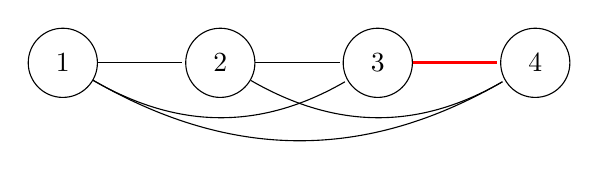
\begin{tikzpicture}[>=stealth',shorten >=1pt, auto, node distance=2cm]
	% Nodes {1, 2, 3, 4}
	\node [state] 	(p1) 				{1};
	\node [state] 	(p2) [right of=p1]  {2};
	\node [state] 	(p3) [right of=p2]  {3};
	\node [state]	(p4) [right of=p3]  {4};
	
	% Paths	{{1, 2}, {2, 3}, {1, 3}, {2, 4}, {1, 4}}
	\path [-] 	(p1) edge (p2)
				(p2) edge (p3)
				(p1) edge[bend right] (p3)
				(p2) edge[bend right] (p4)
				(p1) edge[bend right] (p4)
				(p3) edge[red, very thick] (p4);
\end{tikzpicture}

\noindent
0.9 Write a formal description of the following graph. \\

G = (V, E) where V = \{1, 2, 3, 4, 5, 6\} and \\
\indent
E = \{(1,4), (1,5), (1,6), (2,4), (2,5), (2,6), (3,4), (3,5),(3,6)\} \\

Drawn in Latex this would be: \\ \\

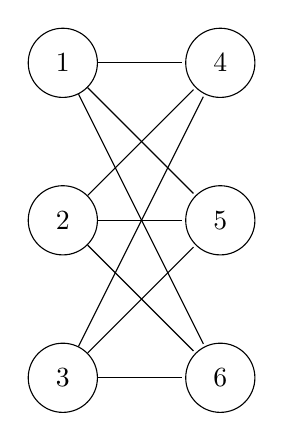
\begin{tikzpicture}[>=stealth',shorten >=1pt, auto, node distance=2cm]
	% Nodes {1, 2, 3, 4}
	\node [state] 	(p1) 				{1};
	\node [state] 	(p2) [below of=p1] 	{2};
	\node [state] 	(p3) [below of=p2]  {3};
	\node [state]	(p4) [right of=p1]  {4};
	\node [state]   (p5) [right of=p2]  {5};
	\node [state]   (p6) [right of=p3]  {6};
	
	% Paths	{(1,4), (1,5), (1,6), (2,4), (2,5), (2,6), (3,4), (3,5),(3,6)}
	\path [-]	(p1) edge (p4)
				(p1) edge (p5)
				(p1) edge (p6)
				(p2) edge (p4)
				(p2) edge (p5)
				(p2) edge (p6)
				(p3) edge (p4)
				(p3) edge (p5)
				(p3) edge (p6);
\end{tikzpicture}

\end{document}
